\documentclass[12pt]{article}

\usepackage{amsmath,amsthm,amssymb,amscd,epsfig,url}
\usepackage{fullpage}
\usepackage{times}
\usepackage{mathdots}
\newtheorem{theorem}{Theorem}[section]
\newtheorem{lemma}[theorem]{Lemma}
\newtheorem{proposition}[theorem]{Proposition}
\newtheorem{corollary}[theorem]{Corollary}
\newtheorem{conjecture}[theorem]{Conjecture}
\newtheorem{definition}[theorem]{Definition}
\newtheorem{example}[theorem]{Example}
\newtheorem{remark}[theorem]{Remark}

\usepackage{xcolor}
\usepackage{tikz}
\usetikzlibrary{arrows.meta, automata, positioning}

\def\ZZ{{\mathbb Z}}
\def\QQ{{\mathbb Q}}
\def\RR{{\mathbb R}}
\def\TT{{\mathcal{C} T}}
\def\KK{{\mathcal{C} K}}
\newcommand{\hus}{\hfill\break}
\newcommand{\bull}{\textbullet\;\;}
\def\iso{{\operatorname{\ \approx \ }}}   % isomorphism
\def\im{{\operatorname{im}}}              % image
\def\Hom{{\operatorname{Hom}}}           % homomorphisms
\def\line{{\operatorname{line} \,}}       % line graph
\def\sd{{\operatorname{sd \,}}}           % first edge subdivision graph
\def\coker{{\operatorname{coker}}}        % cokernel
\def\lcm{{\operatorname{lcm}}}             % least common multiple
\newcommand{\gcdd}{\gamma}              
\def\del{{\partial}}                      % signed incidence matrix
\def\<{{\langle}} \def\>{{\rangle}}       % Inner product
\def\ZC{{Z^\#}}                           % cycle space
\setlength{\textheight}{9in}               
%\setlength{\textwidth}{6in}               % width of text
%\setlength{\oddsidemargin}{0in}           % odd page left margin
%\setlength{\evensidemargin}{0in}          % even page left margin 

\title{Problem Set 2}
\author{CMSC 27230: Honors Theory of Algorithms}
\date{Assigned January 10, 2026, Due January 26, 2026}

\begin{document}
\maketitle

\thispagestyle{empty}
\section*{Problem 0: Collaborators and Outside Sources}
Who were your collaborators (if any)? Which outside sources (if any) did you use?
\section*{Problem 1: Dijkstra's Algorithm}
Use Dijkstra's algorithm to find the shortest path from $s$ to $t$ in the following graph $G$.
    \begin{center}
    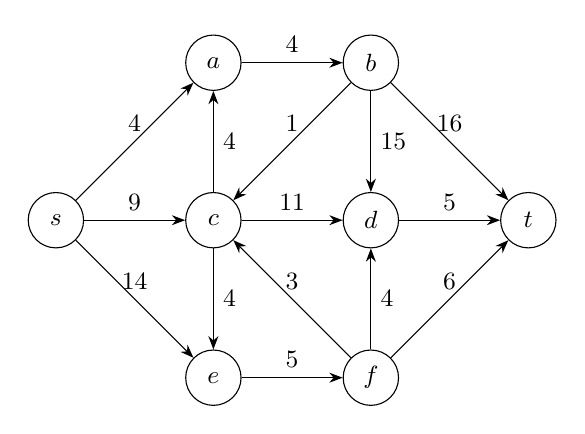
\begin{tikzpicture}[
      mycircle/.style={
         circle,
         draw=black,
         fill=white,
         fill opacity = 0.3,
         text opacity=1,
         inner sep=0pt,
         minimum size=20pt,
         font=\small},
      myarrow/.style={-Stealth},
      node distance=0.6cm and 1.2cm
      ]
      \node[mycircle]  at (-3, 0) (s) {$s$};
      \node[mycircle]  at (-1, 2) (a) {$a$};
      \node[mycircle]  at (1, 2) (b) {$b$};
      \node[mycircle]  at (-1, 0) (c) {$c$};
      \node[mycircle]  at (1, 0) (d) {$d$};
      \node[mycircle]  at (-1, -2) (e) {$e$};
      \node[mycircle]  at (1, -2) (f) {$f$};
      \node[mycircle]  at (3, 0) (t) {$t$};

    \foreach \i/\j/\txt/\p/\pp in {% start node/end node/text/position
      s.45/a.225/4/above/0.5,
      s.00/c.180/9/above/0.5,
      s.315/e.135/14/above/0.5,
      c.90/a.270/4/right/0.5,
      c.270/e.90/4/right/0.5,
      a.00/b.180/4/above/0.5,
      c.00/d.180/11/above/0.5,
      e.00/f.180/5/above/0.5,
      b.225/c.45/1/above/0.5,
      f.135/c.315/3/above/0.5,
      b.270/d.90/15/right/0.5,
      f.90/d.270/4/right/0.5,
      b.315/t.135/16/above/0.5,
      d.00/t.180/5/above/0.5,
      f.45/t.225/6/above/0.5
      }
       \draw [myarrow] (\i) -- node[font=\small,\p,pos=\pp] {\txt} (\j);

    \end{tikzpicture}
    \end{center}
For your answer, first give the state of the priority queue after we add in the edges going out from $s$. Then give the following data for each new vertex that is reached.
\begin{enumerate}
\item The name of the vertex $v$ which is reached and the length of the shortest path from $s$ to $v$.
\item The state of the priority queue after we add in the edges which go out from $v$.
\end{enumerate}
After giving this data, give all of the shortest paths from $s$ to $t$.\\
\\
Note: For this problem, you do not need to show the heap structure of the priority queue. Instead, you can represent the priority queue as a sorted list. Also, you may use either a priority queue with edges or a priority queue with vertices (where the value for a vertex decreases when a shorter path to that vertex is found).\\ 
Note: To find all of the shortest paths from $s$ to $t$, it is useful to record all of the edges $(u,v) \in E(G)$ which can be the final edge of a minimum length path from $s$ to a given vertex $v$.
\section*{Problem 2: True/False Questions (20 points)}
For each of the following statements, state whether the statement is true or false. If the statement is true, explain why it is true. If the statement is false, give a counterexample.
\begin{enumerate}
\item [(a)] Let $G$ be a directed graph where each edge $e \in E(G)$ has a length $l_e \geq 0$. Let $s,t \in V(G)$ be vertices of $G$ and let $P$ be a minimum length path from $s$ to $t$ in $G$. If we increase the length of each edge of $G$ by $2$ then $P$ is still a minimum length path from $s$ to $t$ in $G$.
\item [(b)] Let $G$ be a connected undirected graph where each edge $e \in E(G)$ has a length $l_e \geq 0$ and the lengths of the edges of $G$ are all distinct. Let $T$ be the minimum spanning tree of $G$. If we increase the length of each edge of $G$ by $2$ then $T$ is still the minimum spanning tree of $G$.
\item [(c)] Let $G$ be a connected undirected graph where each edge $e \in E(G)$ has a length $l_e \geq 0$ and the lengths of the edges of $G$ are all distinct. Let $T$ be the minimum spanning tree of $G$. If $e = \{u,v\} \in E(G)$ is an edge such that $e$ is the longest edge incident to $u$ and $e$ is the longest edge incident to $v$ then $e \notin T$.
\item [(d)] Let $G = (V,E)$ and $G' = (V,E')$ be two connected undirected graphs on the same set of vertices $V$ where each edge $e \in E$ has a length $l_e$, each edge $e \in E'$ has a length $l'_e$, and all of these edge lengths are distinct. Let $G''$ be the graph $G'' = (V,E \cup E')$ where edges $e \in E \setminus E'$ have length $l_e$, edges $e \in E' \setminus E$ have length $l'_e$, and edges $e \in E \cap E'$ have length $\min{\{l_e,l'_e\}}$. Letting $T$, $T'$, and $T''$ be the minimum spanning trees of $G$, $G'$, and $G''$ respectively, $T'' \subseteq T \cup T'$ (i.e., every edge in $T''$ is either in $T$ or $T'$).
\end{enumerate}
\section*{Problem 3: Guarding the Vault (20 points)}
You are in charge of guarding a vault. You would like to take a vacation from time $0$ to time $T$, but first you need to hire other guards to guard the vault while you are away (it is okay if more than one person is guarding the vault, but the vault must be guarded at all times). You know $n$ guards you could call, each of whom has a set time interval $[a_i,b_i]$ when they can come and guard the vault. For all $t \in [0,T]$, there is at least one $i$ such that $t \in [a_i,b_i]$. Each guard charges the same amount regardless of the length of their interval $[a_i,b_i]$, so you would like to hire as few guards as possible.

Note: We can state this problem mathematically as follows. Find a set $I \subseteq [n]$ such that $[0,t] \subseteq \cup_{i \in I}{[a_i,b_i]}$ and $|I|$ is minimized.

\begin{enumerate}
\item[(a)] 8 points: Give a greedy algorithm for finding a set of guards to hire so that the number of guards hired is minimized.
\item[(b)] 10 points: Prove that your algorithm is correct.
\item[(c)] 2 points: Explain how to implement your algorithm efficiently and analyze its runtime.
\end{enumerate}
\section*{Problem 4: Restaurant Rush (Rephrasing of Problem 13 in Chapter 4 of Kleinberg-Tardos) (20 points)}
You are the owner of a restaurant and there is suddenly a rush of hungry people. Unfortunately, there is currently only one chef in the kitchen so the people are going to have to wait for a while, but you'd like to minimize the total unhappiness.

To model this problem assume that there are $n$ tables. The orders for table $i$ will take time $l_i > 0$ to cook. If their orders come at a time $t_i$, the total unhappiness of table $i$ will be ${u_i}{t_i}$ where $u_i > 0$. Your goal is to minimize the total unhappiness $\sum_{i=1}^{n}{{u_i}{t_i}}$ where 
\[
t_i = l_i + \sum_{j: \text{Table } j \text{ is served before table } i}{l_j}.
\]
\begin{enumerate}
\item[(a)] 8 points: Give a greedy algorithm for choosing an order to serve the tables in so that the total unhappiness is minimized.
\item[(b)] 10 points: Prove that your algorithm is correct.
\item[(c)] 2 points: Analyze the runtime of your algorithm.
\end{enumerate}
\section*{Problem 5: A Pebble Game (20 points)}
Two players are playing the following pebble game. There is a collection of pebbles of different colors. On each of his/her turns, a player takes all of the pebbles of any one color. Each player aims to maximize the number of pebbles they take.
\begin{enumerate}
\item[(a)] 5 points: Assuming that each pebble only has one color, give an optimal greedy strategy. 
\item[(b)] 10 points: Prove that your answer is correct by showing that if both players follow this strategy, neither player can benefit by deviating from it.
\item[(c)] 5 points: If pebbles can have more than one color, is this strategy still optimal? Either prove that it is still optimal or give a counterexample. Hint is available.
\end{enumerate}
\newpage
\noindent Hints:\\
5c. While the strategy in part a is optimal, sometimes less greedy moves may be equally good. Start with a situation where each pebble only has one color but a less greedy move is just as good as the greediest move and then add more colors to make the less greedy move better.

\end{document}
